\chapter{Baseline Evaluation Results}
\label{ch:baseline_evaluation_results}
This chapter evaluates the original CloudSentinel workflow, before the redesign described in Chapter~9. Online Boutique is used as a new monitored application. The chapter reports the work needed to connect it, two controlled CPU-stress scenarios, and the limitations found in anomaly detection and root-cause analysis (RCA). Chapter~8 translates these findings into design requirements.

\section{Online Boutique: onboarding and setup}
Online Boutique was the first application connected to CloudSentinel outside its original Server Machine Dataset (SMD) and Sock Shop example. It is a Kubernetes microservice application monitored by Prometheus. The onboarding test asks whether the original framework can be moved to this new application and what manual work that requires.

\subsection{Deployment and connectivity}
CloudSentinel was deployed using the provided Kubernetes manifests. Prometheus was deployed through the \texttt{prometheus-community} Helm chart. To connect CloudSentinel to the monitoring stack, the Prometheus endpoint was configured manually through the CloudSentinel interface. In this deployment, the endpoint was \texttt{http://127.0.0.1:55725}.

An additional namespace change was required. The \texttt{CLUSTER\_NAMESPACE} value in the monitoring deployment configuration was changed from \texttt{cloudsentinel} to \texttt{default}, because Online Boutique was deployed in the default namespace. Without this change, CloudSentinel could not identify the relevant application pods.

\subsection{Metric selection and data preparation}
CloudSentinel's original datasets and examples could not be used directly for Online Boutique. Relevant Prometheus metrics were selected and aggregated at pod level: CPU usage, CPU throttling, memory usage, and pod restart rate. The load-generator pod was excluded because it generated workload rather than representing an application component to be monitored.

The selected metrics were exported from Prometheus and prepared with custom scripts. The scripts aligned timestamps and converted the data into CloudSentinel's required training, test, and label files. The training file represented normal behaviour. The test file included the recorded fault period, and its labels marked which timestamps belonged to that period. A model could not be trained or evaluated until these steps were completed.

\subsection{Configuration and manual intervention}
Several steps required manual work. Besides changing the Prometheus address and namespace, Online Boutique needed new metric mappings. The trained model also had to be made available to Live Monitoring. Settings entered through the interface did not always reach the services that collected data or ran the model. The active configuration therefore had to be checked and sometimes corrected manually.

The onboarding result shows that CloudSentinel can be configured for a new environment. However, the required settings, scripts, and manual corrections were spread across several places. The original workflow was therefore not yet self-contained or straightforward to reproduce.

\subsection{Summary of onboarding effort}
Table~\ref{tab:online_boutique_onboarding} summarises the main onboarding activities. The table records practical effort rather than precise time measurements, as the setup process was iterative and included troubleshooting.

\begin{table}[htbp]
    \centering
    \small
    \caption{Main onboarding activities for Online Boutique.}
    \label{tab:online_boutique_onboarding}
    \begin{tabular}{p{0.28\textwidth} p{0.30\textwidth} p{0.30\textwidth}}
        \toprule
        \textbf{Activity} & \textbf{File or configuration} & \textbf{Observed friction} \\
        \midrule
        Deploy framework and monitoring stack & Kubernetes manifests and Prometheus Helm chart & Components had to be configured separately. \\
        Configure monitoring access & Prometheus endpoint and namespace setting & Default namespace configuration did not match Online Boutique. \\
        Select and map metrics & Prometheus queries and pod-level feature set & Original examples did not match Online Boutique services or labels. \\
        Prepare datasets & Custom export, alignment, reshaping, and labelling scripts & Manual work was needed to construct training, testing, and label arrays. \\
        Configure live workflow & Trained model and monitoring configuration & Configuration propagation required manual checking and correction. \\
        \bottomrule
    \end{tabular}
\end{table}

The results show that the original CloudSentinel could be connected to Online Boutique, but only after several environment-specific and manual steps. The main difficulty was not deploying one component. It was keeping the Prometheus address, namespace, metric mapping, prepared files, model, and Live Monitoring settings consistent across the workflow. This onboarding result therefore supports limited portability, rather than a claim of simple plug-and-play deployment.

\section{Online Boutique: end-to-end workflow under controlled interventions}
This section reports two controlled CPU-stress scenarios. Each scenario follows the same order: the injected fault, the Live Monitoring response, the RCA result, and a later replay of the saved data. This makes it possible to distinguish successful workflow execution from accurate detection or diagnosis.

\subsection{Interpreting the CloudSentinel monitoring output}
Two related tests were used. First, Live Monitoring checked whether CloudSentinel could repeatedly retrieve recent Prometheus data and run the selected model. The interface displayed the percentage of evaluated timestamps marked anomalous. RCA started when this percentage crossed the configured RCA trigger.

Second, saved Prometheus data were processed after the experiment. This is called \textit{manual replay}. It produced one normal-or-anomalous decision for every timestamp that the model could evaluate. Because the fault period was known, these decisions could be compared with labels for normal and faulty operation. Precision shows how many reported anomalies were correct, recall shows how much of the labelled fault period was found, and F1 combines both.

CloudSentinel uses a forecasting-based detector. It uses earlier observations to predict the following metric values. The difference between the prediction and the actual values becomes an anomaly score. The model also stores an anomaly cut-off, called \texttt{epsilon} in the implementation. A timestamp is marked anomalous when its score reaches this cut-off.

The percentage shown in the Live Monitoring graph is not a probability or a measure of fault severity. It is the share of evaluated timestamps in the current window that crossed the model's anomaly cut-off. For example, 14.286\% means that approximately one in seven evaluated timestamps was marked anomalous. RCA starts when this percentage exceeds the configured RCA trigger.

The model needs earlier observations before it can make its first prediction. This earlier part is called the lookback window. With the configured lookback of 100 observations, the first 100 input timestamps provide context and do not receive a prediction. These are the warm-up observations.

Live Monitoring and manual replay use the same model but do not prepare their input in exactly the same way. Training rescales values using the range found in the training data. A later detection request instead calculates a new range from the data submitted in that request. Live Monitoring repeatedly submits new windows, so the same raw value can be rescaled differently over time. This limits direct comparison between the graph and the manual replay below.

\subsection{Single-pod CPU stress on \texttt{paymentservice}}
\subsubsection{Fault injection and setup}
This scenario examined whether CloudSentinel could detect CPU pressure affecting one service pod and whether the subsequent RCA output would identify \texttt{paymentservice} or its related metrics as relevant candidates.

Table~\ref{tab:paymentservice-cpu-setup} summarises the scenario configuration.

\begin{table}[htbp]
    \centering
    \small
    \caption{Configuration of the single-pod CPU-stress scenario.}
    \label{tab:paymentservice-cpu-setup}
    \begin{tabular}{l l}
        \toprule
        \textbf{Item} & \textbf{Value} \\
        \midrule
        Target component & \texttt{paymentservice} \\
        Fault mechanism & CPU-intensive \texttt{yes} process in an ephemeral debug container \\
        Fault start & 15:20 UTC (17:20 local time) \\
        Fault end & 15:45 UTC (17:45 local time) \\
        Monitoring data window & 16:35--18:15 local time \\
        Live-monitoring duration & 30 minutes \\
        \bottomrule
    \end{tabular}
\end{table}

The fault was injected by starting a CPU-intensive \texttt{yes} process in an ephemeral BusyBox debug container attached to the \texttt{paymentservice} pod. The process continuously consumed CPU resources. The \texttt{wait} command kept the shell session active until the process was terminated.

\begin{verbatim}
kubectl debug pod/paymentservice -it --image=busybox:1.36 \
-- sh -c 'yes > /dev/null & wait'
\end{verbatim}

\subsubsection{Live-monitoring result}
Figure~\ref{fig:paymentservice-cpu-live} shows the live anomaly percentage during the CPU-stress injection. The percentage increased shortly after the stress process was started, crossed the configured 4\% RCA threshold several times, and decreased after the process was stopped. This shows that the live workflow responded to the intervention: Prometheus data were collected, CloudSentinel produced an anomaly percentage, the threshold triggered RCA, and RCA output was displayed.

A temporary dip was visible around 17:31 local time even though CPU stress was still active. This confirms that the percentage should not be read as a direct measure of fault severity. The scenario interpretation below explains likely reasons.

\begin{figure}[htbp]
    \centering
    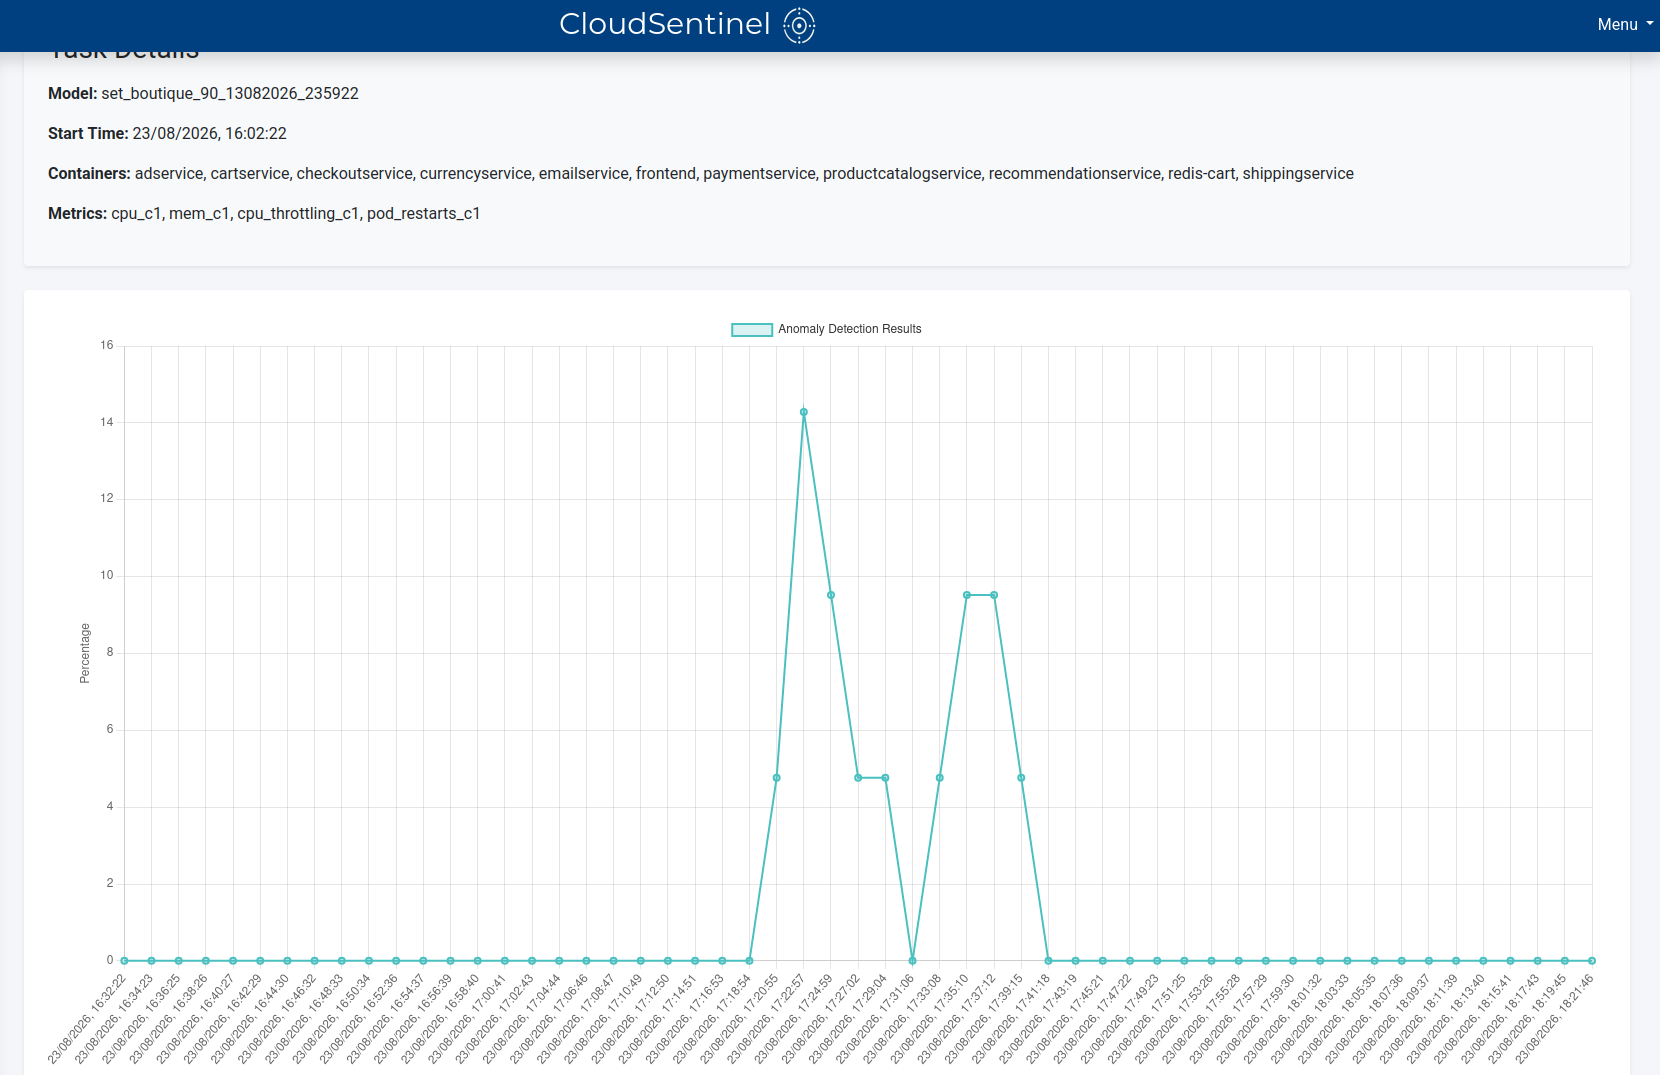
\includegraphics[width=\textwidth]{figures/boutique/scenario1/live_monitoring_graph_data.png}
    \caption{CloudSentinel Live Monitoring view during CPU stress injected into \texttt{paymentservice}. The fault was active from 17:20 to 17:45 local time. Each graph value is the percentage of evaluated timestamps marked anomalous in that update.}
    \label{fig:paymentservice-cpu-live}
\end{figure}

A UI-related issue was observed during this session. Live monitoring was started at approximately 16:35 local time, but the interface displayed a session timestamp of 16:02:22. The displayed time therefore appeared to be offset by approximately the configured 30-minute monitoring duration. Interface timestamps could not be directly interpreted as actual execution times without manually comparing them with the recorded fault-injection times.

\subsubsection{RCA result}
RCA was triggered nine times during the session. These events corresponded to the nine displayed anomaly percentages above the 4\% RCA threshold. The first RCA execution occurred at approximately 17:20 local time, shortly after the CPU-stress injection started, and was associated with an anomaly percentage of 4.762\%. In the interface dropdown, however, this event was displayed with timestamp 16:50:55, again indicating an offset close to the configured monitoring duration.

The first RCA ranking contained some useful evidence but did not clearly identify the affected service. Payment-service CPU throttling ranked second and payment-service memory ranked third. However, direct payment-service CPU use ranked only 26th, while an unrelated currency-service CPU metric ranked first.

The highest anomaly percentage observed during the session was 14.286\%. Despite this stronger anomaly signal, the corresponding RCA ranking represented \texttt{paymentservice} less clearly. The relevant pod-restart, CPU, CPU-throttling, and memory metrics ranked between positions 22 and 34.

Table~\ref{tab:paymentservice-cpu-rca} summarises three representative RCA events: the first trigger, the event with the highest anomaly percentage, and the final observed trigger.

\begin{table}[htbp]
    \centering
    \scriptsize
    \caption{Selected RCA results during single-pod CPU stress on \texttt{paymentservice}.}
    \label{tab:paymentservice-cpu-rca}
    \begin{tabularx}{\textwidth}{l c X X}
        \toprule
        \textbf{RCA event} & \textbf{Anomaly percentage} & \textbf{Relevant \texttt{paymentservice} output} & \textbf{Interpretation} \\
        \midrule
        First RCA trigger
        & 4.762\%
        & CPU throttling: rank 2, score 0.08084; memory: rank 3, score 0.03491; pod restarts: rank 21; CPU: rank 26, score 0.02622
        & Some relevant metrics were ranked prominently, but direct CPU usage was low-ranked. \\

        Highest anomaly trigger
        & 14.286\%
        & Pod restarts: rank 22, score 0.02701; CPU: rank 29, score 0.02260; CPU throttling: rank 30, score 0.01838; memory: rank 34, score 0.01222
        & The affected service was weakly represented despite the strongest observed anomaly percentage. \\

        Last observed RCA trigger
        & Not recorded separately
        & Pod restarts: rank 26; memory: rank 27; CPU: rank 29; CPU throttling: rank 31
        & Relevant metrics were low-ranked; RCA did not reliably localise the affected component. \\
        \bottomrule
    \end{tabularx}
\end{table}

\subsubsection{Manual replay result}
The manual replay used the exported monitoring data to produce an anomaly score and a normal-or-anomalous decision for every timestamp the model could evaluate. The detailed output was stored in \texttt{scenario\_prediction\_output.csv}.

A separate script compared these decisions with labels derived from the recorded CPU-stress period. A true positive (TP) is a fault timestamp correctly marked anomalous; a false positive (FP) is a normal timestamp marked anomalous. A true negative (TN) is a normal timestamp correctly marked normal, and a false negative (FN) is a fault timestamp that the detector missed. These counts were used to calculate precision, recall, and F1.

The input data contained 381 timestamps. Because the model used a lookback of 100 timestamps, manual detection generated 281 aligned output predictions. Within this aligned window, 101 timestamps were labelled as part of the CPU-stress interval and 180 timestamps were labelled as normal operation.

The saved anomaly cut-off was evaluated first. Two lower cut-offs were then explored to see whether the result was sensitive to this setting. The model, data, labels, and timestamp alignment stayed the same; only the cut-off between a normal and anomalous decision changed.

Table~\ref{tab:paymentservice-cpu-manual} summarises the manual replay results.

\begin{table}[htbp]
    \centering
    \small
    \caption{Exploratory manual replay results for the single-pod CPU-stress scenario.}
    \label{tab:paymentservice-cpu-manual}
    \begin{tabular}{l r r r r r r r}
        \toprule
        \textbf{Threshold} & \textbf{TP} & \textbf{FP} & \textbf{TN} & \textbf{FN} & \textbf{Precision} & \textbf{Recall} & \textbf{F1} \\
        \midrule
        Stored anomaly cut-off: 0.1488
        & 0 & 0 & 180 & 101 & N/A & 0.000 & N/A \\
        Exploratory cut-off: 0.125
        & 5 & 0 & 180 & 96 & 1.000 & 0.050 & 0.094 \\
        Exploratory cut-off: 0.100
        & 30 & 13 & 167 & 71 & 0.698 & 0.297 & 0.417 \\
        \bottomrule
    \end{tabular}
\end{table}

At the stored anomaly cut-off of 0.1488, manual detection did not classify any of the 281 aligned timestamps as anomalous. All 101 timestamps belonging to the recorded CPU-stress interval were classified as normal. Lowering the cut-off produced some detections within the fault interval, but the resulting signal remained incomplete. At 0.125, only five fault-labelled timestamps were detected. At 0.100, recall increased to 0.297, but 13 normal timestamps were also classified as anomalous.

The two lower cut-offs were chosen after viewing this scenario. They therefore show only how sensitive the outcome is to the cut-off and are not treated as independently selected model settings. The result for the saved model remains that manual replay detected none of the labelled fault timestamps.

\subsubsection{Scenario interpretation}

The results show that the original end-to-end workflow could respond to an injected fault: the Live Monitoring percentage increased, RCA started, and the percentage later decreased. This demonstrates workflow execution, not reliable detection accuracy.

Manual replay did not show reliable detection for individual timestamps under the saved configuration. It also cannot be equated directly with the Live Monitoring graph. Live Monitoring reports one percentage for each recent window, whereas manual replay evaluates individual timestamps in one saved dataset.

Different input scaling further limits direct comparison. Training determines its value range from the training data, while a later detection request determines a new range from its own input window. The saved anomaly cut-off does not change with that range. A raw metric value can therefore lead to a different internal value, making decisions difficult to compare across Live Monitoring windows and manual replay.

The RCA output was also inconclusive. RCA was triggered during the fault interval and some \texttt{paymentservice}-related metrics appeared in the ranking. However, the directly stressed service was not consistently prioritised. The scenario therefore provides evidence of workflow feasibility and partial representation of the affected component, rather than reliable root-cause localisation.

\subsection{Sequential multi-pod CPU stress}

\subsubsection{Fault injection and setup}

The second scenario applied CPU stress independently to five Online Boutique services: \texttt{paymentservice}, \texttt{shippingservice}, \texttt{emailservice}, \texttt{cartservice}, and \texttt{checkoutservice}. The injections were started five minutes apart. This produced a stronger and more distributed disturbance than the single-pod scenario.

The sequence was selected to cover several services involved in the Online Boutique request workflow. However, CPU stress was injected independently into every pod. It did not represent a real application-level fault propagating from one service to another. The scenario can therefore show how CloudSentinel reacts to distributed stress, but it cannot validate reconstruction of a genuine causal chain.

Table~\ref{tab:multipod-cpu-setup} summarises the scenario configuration.

\begin{table}[htbp]
    \centering
    \small
    \caption{Configuration of the multi-pod CPU-stress scenario.}
    \label{tab:multipod-cpu-setup}
    \begin{tabular}{l l}
        \toprule
        \textbf{Item} & \textbf{Value} \\
        \midrule
        Target components & \texttt{paymentservice}, \texttt{shippingservice}, \texttt{emailservice}, \texttt{cartservice}, and \texttt{checkoutservice} \\
        Fault mechanism & CPU-intensive \texttt{yes} process in an ephemeral debug container for each target pod \\
        First fault start & 13:40 UTC (15:40 local time) \\
        Injection interval & Five minutes between starting each stress process \\
        Monitoring data window & 15:00--19:21 local time \\
        Live-monitoring duration & 30 minutes \\
        \bottomrule
    \end{tabular}
\end{table}

For each target pod, a CPU-intensive process was started in an ephemeral debug container. The processes were terminated sequentially in reverse order, with five minutes between terminations.

\begin{verbatim}
kubectl debug pod/[PODNAME] -it --image=busybox:1.36 \
-- sh -c 'yes > /dev/null & wait'
\end{verbatim}

\subsubsection{Live-monitoring result}

Figure~\ref{fig:multipod-livemonitoring-cpu-live} shows the live anomaly percentage during the multi-pod scenario. The percentage reached a maximum of 57.143\%. RCA was triggered 67 times while the CPU-stress processes were active. This was a stronger live response than in the single-pod scenario.

The graph also contained repeated dips. At some points it returned to 0\% even though CPU stress was still active. The percentage therefore did not represent the severity or continued presence of the fault directly.

\begin{figure}[htbp]
    \centering
    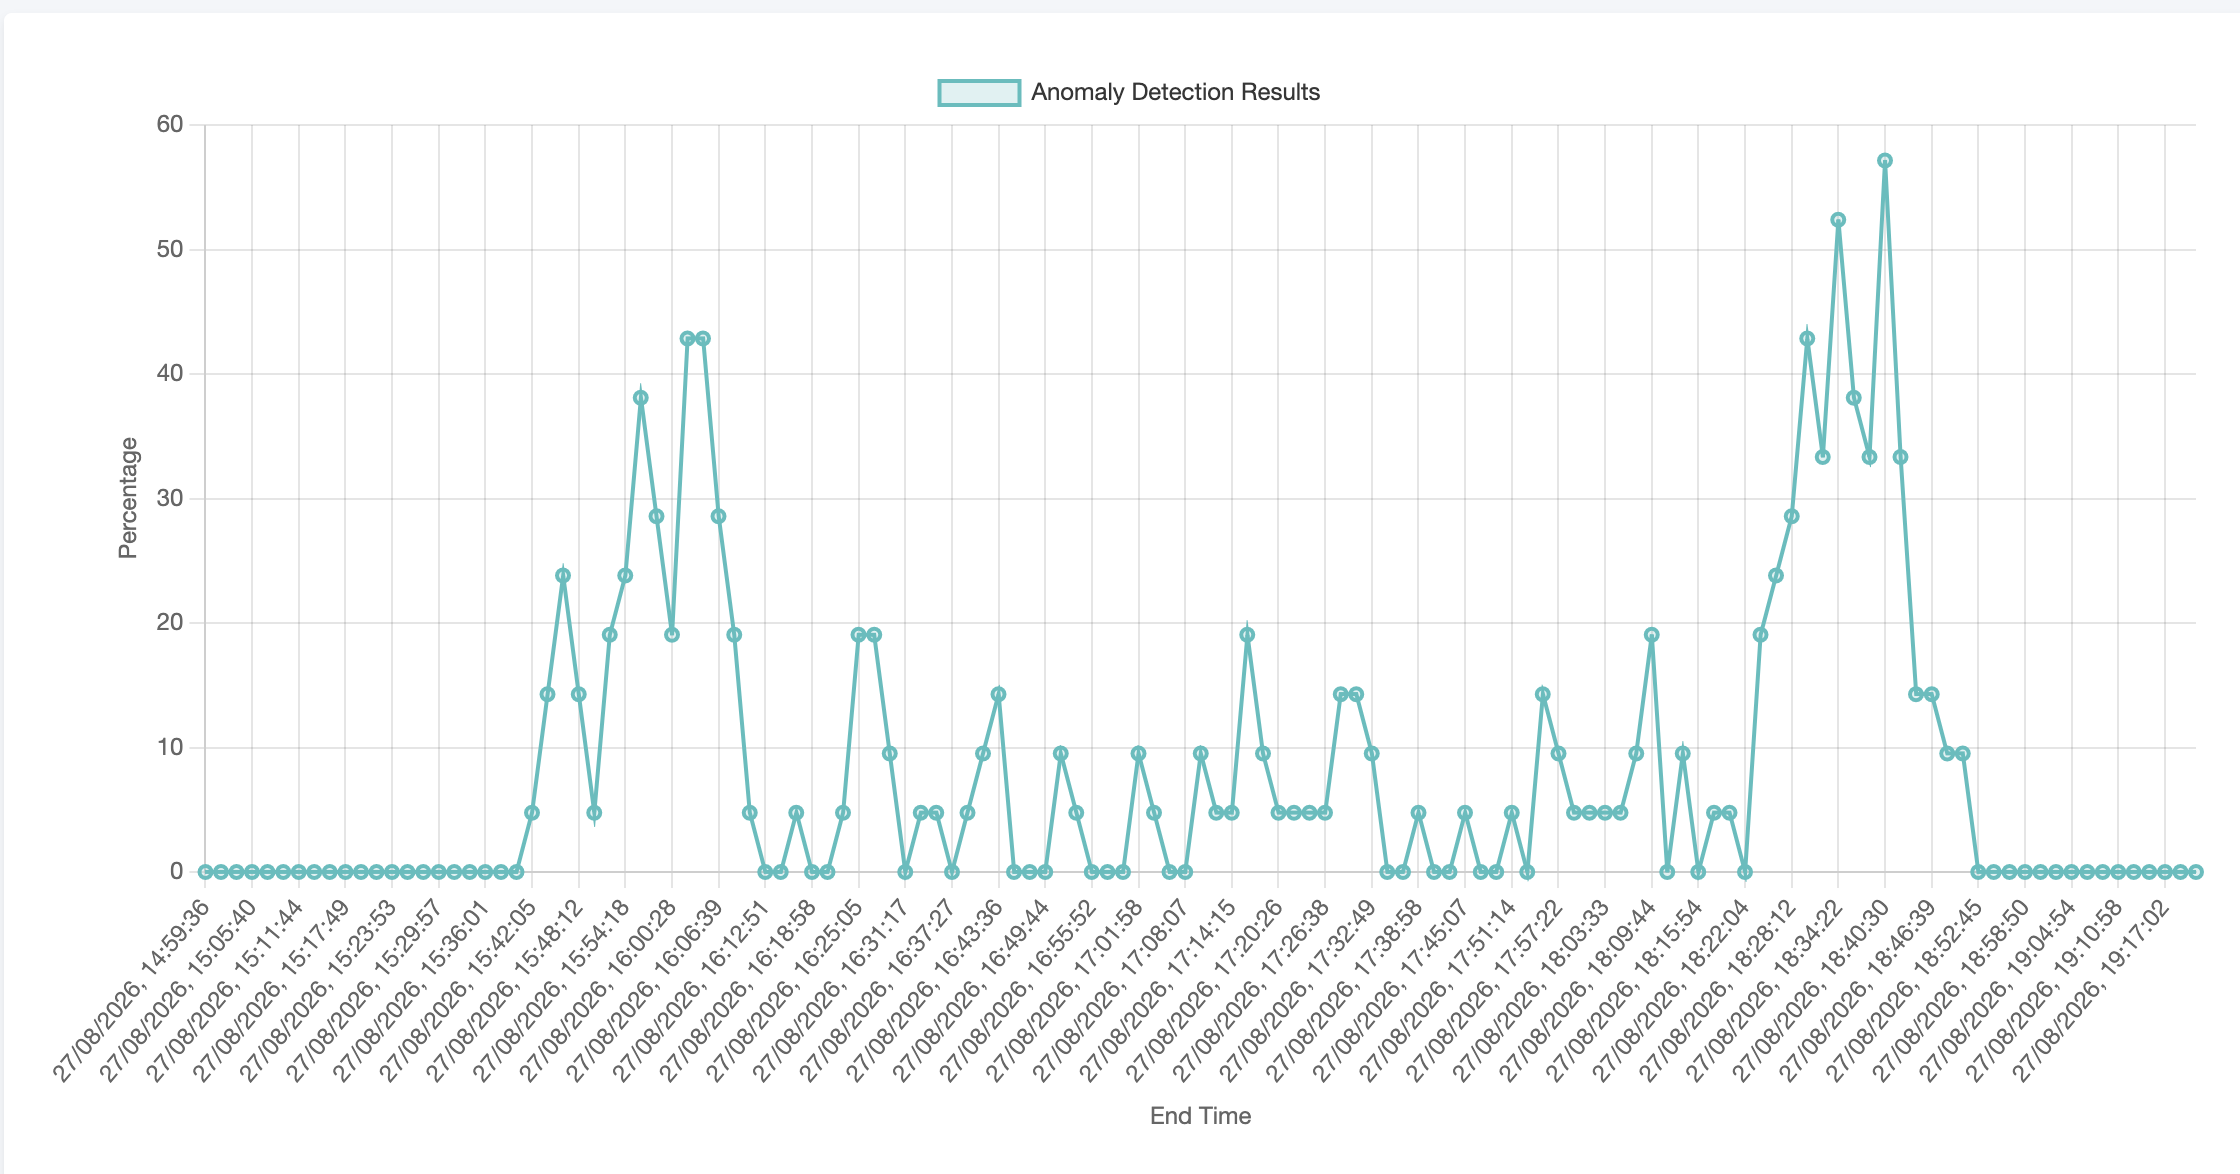
\includegraphics[width=\textwidth]{figures/boutique/scenario2/scenario2_graph_result.png}
    \caption{CloudSentinel Live Monitoring view during sequential CPU stress on five Online Boutique services. Each graph value is the percentage of evaluated timestamps marked anomalous in that update.}
    \label{fig:multipod-livemonitoring-cpu-live}
\end{figure}

The detector's forecasting design offers one possible explanation. At the start of CPU stress, its recent context mainly contains normal behaviour, so the new high values are difficult to predict and receive high anomaly scores. Later, the recent context itself contains stressed observations. A stable high-CPU state can then become easier to predict even though it is still operationally abnormal.

The model is not retrained during this process; only its recent input window changes. Removing the stress can create another prediction error because the recent context still contains high CPU values. This explanation fits the graph, but the experiment did not isolate it from other influences such as input scaling.

The changing input scale described earlier may strengthen this effect. Each detection request calculates a new range for its own window, while the saved anomaly cut-off remains fixed. This makes the Live Monitoring percentage harder to interpret consistently.

\subsubsection{RCA result}
RCA was first triggered at approximately 15:42 local time, with an anomaly percentage of 4.762\%. The first RCA ranking did not show a clear causal ordering of the injected services. \texttt{frontend\_cpu} ranked first, followed by \texttt{paymentservice\_cpu}, \texttt{checkoutservice\_cpu}, and several checkoutservice-related features. Other relevant metrics were ranked much lower. For example, \texttt{paymentservice\_cpu\_throttling} ranked 32nd.

The highest anomaly percentage observed during the session occurred at approximately 18:40 local time and was 57.143\%. This event also did not identify \texttt{paymentservice}, or another clearly defined initiating service, as a clear root cause. The rankings remained dispersed across multiple services and metrics.

The RCA results therefore show that the framework can trigger and produce RCA output during a distributed disturbance. They do not show that CloudSentinel reconstructed the intended injection sequence or identified one genuine causal origin.

\subsubsection{Manual replay result}

Table~\ref{tab:multipod-manual-detection-results} summarises the manual replay results for the multi-pod scenario.

\begin{table}[htbp]
    \centering
    \small
    \caption{Manual replay results for the multi-pod CPU-stress scenario.}
    \label{tab:multipod-manual-detection-results}
    \begin{tabular}{r r r r r r r r}
        \toprule
        \textbf{Aligned rows} & \textbf{TP} & \textbf{FP} & \textbf{TN} & \textbf{FN} & \textbf{Precision} & \textbf{Recall} & \textbf{F1} \\
        \midrule
        925 & 9 & 0 & 200 & 716 & 1.000 & 0.012 & 0.025 \\
        \bottomrule
    \end{tabular}
\end{table}

The manual replay contained 925 aligned timestamps, of which 725 were labelled as part of the multi-pod CPU-stress interval. Only nine of those 725 timestamps were classified as anomalous. No normal timestamps were classified as anomalous, resulting in a precision of 1.000. However, 716 fault-labelled timestamps were classified as normal, resulting in a recall of 0.012 and an F1-score of 0.025.

The perfect precision does not mean that the detector covered the fault well. It made only nine anomalous predictions, and all nine happened during the fault period. It missed the other 716 fault timestamps. The saved configuration therefore detected a few distinctive moments but not the sustained multi-pod stress reliably.

\subsubsection{Scenario interpretation}
The results show that the larger distributed disturbance produced a stronger Live Monitoring response: the percentage reached 57.143\% and RCA started 67 times. This confirms that the end-to-end workflow remained active during the scenario.

At the same time, the repeated dips in the live percentage and the low recall in manual replay show that a high live percentage should not be interpreted as reliable timestamp-level detection of the full stress interval. The forecasting-based input context and the per-window scaling behaviour both limit comparability between monitoring iterations.

The RCA rankings did not identify a clear initiating component. This outcome is partly expected because the injected CPU stress was concurrent and independently applied to multiple pods. The scenario is therefore evidence of workflow behaviour and RCA interpretability under distributed stress, rather than a valid causal-chain benchmark.

\subsection{Cross-scenario workflow summary}
Table~\ref{tab:online_boutique_workflow_summary} summarises the evidence from the two completed scenarios.

\begin{table}[htbp]
    \centering
    \small
    \caption{Cross-scenario workflow summary for Online Boutique.}
    \label{tab:online_boutique_workflow_summary}
    \begin{tabular}{p{0.18\textwidth} p{0.20\textwidth} p{0.15\textwidth} p{0.20\textwidth} p{0.20\textwidth}}
        \toprule
        \textbf{Scenario} & \textbf{Anomaly percentage observed} & \textbf{RCA triggered} & \textbf{Intervention target represented} & \textbf{Interpretation} \\
        \midrule
        Single-pod CPU stress & Yes; percentage increased and crossed the threshold, with an unexplained dip. & Yes; 9 times & Partly; paymentservice-related metrics appeared, but inconsistently. & End-to-end workflow was functional, but localisation was unreliable. \\
        Sequential multi-pod CPU stress & Yes; stronger response, with a maximum of 57.143\%. & Yes; 67 times & Partly; affected and related metrics appeared, but rankings were dispersed. & Framework responded to distributed stress, but output did not identify a clear causal origin. \\
        \bottomrule
    \end{tabular}
\end{table}

Taken together, the results show that the original workflow executed during both interventions: monitoring produced output and RCA was triggered. They do not show reliable fault detection or localisation. The single-pod and multi-pod tests therefore establish technical workflow feasibility while also revealing why the output was difficult to trust and interpret.

\section{Framework limitations revealed by Online Boutique}
The Online Boutique case revealed limitations that are relevant beyond the two individual scenarios. These findings concern the consistency and usability of the framework workflow, rather than only the output of the embedded algorithms.

\subsection{Consistency of input preparation and anomaly cut-offs}
\label{sec:preprocessing_threshold_consistency}
CloudSentinel rescales metric values differently during training and later detection. Training determines the scale from the training data and reuses it for its accompanying test data. A separate detection request determines a new scale from the values in that request. Because Live Monitoring repeatedly sends new recent windows, the scale can change between updates.

The model's anomaly cut-off was calculated using the training scale. Applying that unchanged cut-off to differently scaled data makes results difficult to compare. This is one reason why sustained CPU stress could produce high percentages at transitions but low percentages in the middle of the same fault. It also means that the manual replay scores cannot be used as direct validation of the Live Monitoring graph.

\subsection{Configuration propagation and reproducibility}
The Live Monitoring workflow required additional manual work after training and configuration through the interface. Settings did not always reach the services that collected data or ran the model. Model files and environment-specific settings also required manual handling.

The interface configuration alone was therefore not enough to repeat a successful run. A reproducible workflow should preserve the model, input-preparation settings, metric mapping, and monitoring configuration together.

\subsection{Manual data engineering and application coupling}
Online Boutique could not be connected to CloudSentinel without application-specific metric selection, Prometheus exports, timestamp alignment, reshaping, and label construction. The original datasets and examples did not provide a direct template for the new application.

This work may be acceptable for a controlled research prototype, but it makes repeated experiments and routine use harder. It also shows that CloudSentinel depends on assumptions about metric names, service names, and file structure. Clear metric mappings, reusable data preparation, and automated dataset construction could reduce this coupling.

\subsection{RCA interpretability and fragmented operator workflow}
CloudSentinel and Grafana supported different parts of the diagnostic workflow. Grafana was used to inspect raw metrics and verify the effect of fault injections, while CloudSentinel presented anomaly percentages and RCA rankings. The connection between these views was limited. Users had to manually relate a CloudSentinel result to the relevant service, metric, time period, and system behaviour in Grafana.

The Live Monitoring interface provided limited context. It showed an anomaly percentage without clearly explaining what it represented, which timestamps and metrics contributed, or how to interpret the configured trigger. The session time also appeared to differ from the actual execution time. A user could therefore see the percentage change without understanding why.

RCA output added limited context to this view. It was primarily expressed as ranked metrics rather than as an explanation of the affected service and likely operational cause. The rankings could contain affected metrics, but did not consistently identify the affected service or explain why a metric was considered relevant. This reduced the direct usefulness of the output for an operator.

\subsection{Implications for portability and extensibility}
The baseline evaluation shows that CloudSentinel can be adapted to Online Boutique, but that adaptation is not lightweight. Portability is limited by manual environment-specific configuration and a Prometheus-centred data path. A direct dependency on Prometheus may also limit use in environments that primarily use other observability backends; this latter limitation was not evaluated empirically in the present study.

The evaluation also does not show that anomaly-detection or RCA methods can be replaced easily. Metric preparation, model input, trained files, anomaly cut-offs, and monitoring settings depended on each other. Clear method interfaces and data formats would be needed before the framework could be described as genuinely extensible.

\section{Resource-overhead observations}
[TODO]
% C5 remains preliminary. The baseline evaluation was conducted in a constrained local Minikube cluster, but no systematic comparison of CloudSentinel CPU and memory use during idle and active operation was completed. The available observations are insufficient to support a reliable quantitative overhead claim.

% A focused idle-versus-active CPU and memory measurement can be added after the baseline evaluation is completed. Until then, resource efficiency is treated as a design requirement and as a limitation of the current evidence rather than as a completed result.

\section{NaaVRE portability case}
\label{sec:naavre_results}

NaaVRE was evaluated only after the redesigned workflow and the evaluation-only Grafana adapter existed. It is therefore not part of the original-framework baseline in this chapter. Its protocol is described in Section~\ref{sec:naavre_protocol} and its results are reported with the redesigned workflow in Chapter~9.

\section{Result summary and evidence boundary}
Table~\ref{tab:baseline_evidence_summary} makes the baseline evidence boundary explicit. Online Boutique is the controlled baseline case. The later RCAEval and NaaVRE cases evaluate the redesigned workflow and are therefore kept outside this table.

\begin{table}[htbp]
    \centering
    \small
    \caption{Completed baseline evidence and its scope.}
    \label{tab:baseline_evidence_summary}
    \begin{tabular}{p{0.20\textwidth} p{0.25\textwidth} p{0.22\textwidth} p{0.25\textwidth}}
        \toprule
        \textbf{Case} & \textbf{Evidence completed} & \textbf{Criteria supported} & \textbf{Evidence boundary} \\
        \midrule
        Online Boutique & Onboarding, two controlled CPU-stress scenarios, live workflow observations, RCA output, and manual replay. & C1 (workflow), C2 (RCA), C3 (portability), and C4 (reproducibility); C5 (overhead) remains preliminary. & Controlled local proof of concept; not a broad algorithm benchmark or production deployment. \\
        \bottomrule
    \end{tabular}
\end{table}

The results show that the original CloudSentinel could be connected to a new Kubernetes microservice application and could execute its anomaly-detection and RCA pipeline. They do not show reliable anomaly detection or root-cause localisation. The case instead reveals substantial manual onboarding work, inconsistent input preparation and configuration, and Live Monitoring and RCA output that required considerable interpretation. Chapter~8 evaluates these findings against the five criteria for workflow adequacy, RCA, portability, reproducibility, and operational overhead, and derives requirements for the redesign.
